
\section{\numb section 1. General description}

This section is a quick tour through \maniFEM's capabilities.


\paragraph{\numb section 1.\numb parag 1. An elementary example}

In this paragraph, we show how to build a rectangular mesh on a surface in $ \RR^3 $ 
and then compute the integral of a given function.
Paragraph \numb section 1.\numb parag 3 shows a purely two-dimensional example.

\bigskip
{ \psfrag{SW}{\special{ps: gsave 0 0 0.8 setrgbcolor}{\codett SW}\special{ps: grestore}}
\psfrag{NW}{\special{ps: gsave 0 0 0.8 setrgbcolor}{\codett NW}\special{ps: grestore}}
\psfrag{SE}{\special{ps: gsave 0 0 0.8 setrgbcolor}{\codett SE}\special{ps: grestore}}
\psfrag{NE}{\special{ps: gsave 0 0 0.8 setrgbcolor}{\codett NE}\special{ps: grestore}}
\centerline{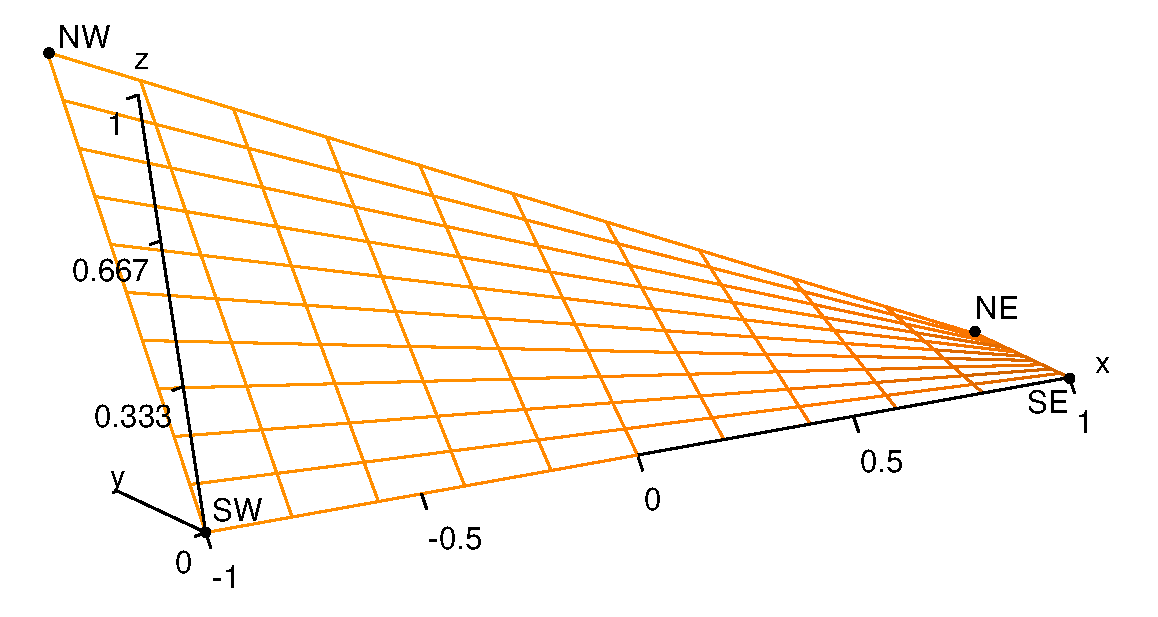
\includegraphics[width=90mm]{3d-rectangle.eps}} }

%\code{\numb section 1.\numb code 1}
\verbatim
#include "maniFEM.h"

using namespace maniFEM;
using namespace std;

int main ()

{  // we choose our (geometric) space dimension :
   Manifold RR3 ( tag::Euclid, tag::of_dim, 3 );
   
   // xyz is a map defined on our future mesh with values in RR3 :
   Function xyz = RR3.build_coordinate_system ( tag::Lagrange, tag::of_degree, 1 );

   // we can extract components of xyz using the [] operator
   Function x = xyz[0],  y = xyz[1],  z = xyz[2];

   // Let's build a rectangular mesh. First, the four corners :
   Cell SW ( tag::vertex );  x(SW) = -1;  y(SW) = 0;  z(SW) = 0;
   Cell SE ( tag::vertex );  x(SE) =  1;  y(SE) = 0;  z(SE) = 0;
   Cell NE ( tag::vertex );  x(NE) =  1;  y(NE) = 1;  z(NE) = 0;
   Cell NW ( tag::vertex );  x(NW) = -1;  y(NW) = 1;  z(NW) = 1;
   
   // we access the coordinates of a point using the () operator :
   cout << "coordinates of NW : " << x(NW) << " " << y(NW) << " " << z(NW) << endl;
   
   // now build the four sides of the rectangle :
   Mesh south ( tag::segment, SW.reverse(), SE, tag::divided_in, 10 );
   Mesh east  ( tag::segment, SE.reverse(), NE, tag::divided_in, 10 );
   Mesh north ( tag::segment, NE.reverse(), NW, tag::divided_in, 10 );
   Mesh west  ( tag::segment, NW.reverse(), SW, tag::divided_in, 10 );
   
   // and now the rectangle :
   Mesh rect_mesh ( tag::rectangle, south, east, north, west );

   // We may want to visualize the resulting mesh.
   // Here is one way to export the mesh in the "msh" format :
   rect_mesh.export_msh ("rectangle.msh");

   // Let's define a symbolic function to integrate
   Function f = x*x+1/(5+y);
   // and compute its integral on the rectangle,
   // using Gauss quadrature with 9 points

   FiniteElement fe
      ( tag::with_master, tag::quadrangle, tag::Lagrange, tag::of_degree, 1 );
   fe.set_integrator ( tag::Gauss, tag::quad_9 );

   // code below does not work yet

   // cout << "integral of " << f.repr() << " = "
   //      << fe.integrate ( f, tag::over, rect_mesh ) << endl;
   // cout << "integral of " << g.repr() << " = "
   //      << fe.integrate ( g, tag::over, rect_mesh ) << endl;

}  // end of main
\endverbatim
%\endcode

To run this example, you will need a recent {\tt C++} compiler and the {\tt make} utility.
Visit {\codett https://github.com/cristian-barbarosie/manifem}
and copy all files under {\codett src/} to some directory in your computer.
Launch the program through the command {\codett make run-\numb section 1.\numb parag 1};
a file {\codett rectangle.msh} should appear in the working directory.
You may view the mesh using the software {\tt gmsh}.

Expressions like {\codett tag::of\_dim} and {\codett tag::vertex} are
objects belonging to the {\codett namespace tag}; we use them as arguments to many functions.
See paragraph \numb section 10.\numb parag 2 for some details.

When declaring a segment {\codett Mesh}, we must {\codett reverse} the first vertex
(paragraph~\numb section 1.\numb parag 2 discusses the {\codett reverse} method).
Paragraph~\numb section 1.\numb parag 3 explains why we build
the rectangle based on its four sides rather than on its four vertices.

Note that in this example we do not have exact control on the shape of the surface being meshed.
The coordinates of the inner vertices are defined rather vaguely by interpolating the
coordinates of the four corners.
See sections \numb section 2 and \numb section 3
for ways to precisely define a submanifold in $ \RR^3 $ and mesh (a bounded domain of) it.


\paragraph{\numb section 1.\numb parag 2. Cells and meshes}

In \maniFEM, all basic constituents of meshes are called ``cells''. 
Points are zero-dimensional cells, segments are one-dimensional cells, triangles are
two-dimensional cells, and so on.

Roughly speaking, a mesh is a collection of cells of the same dimension. 
For efficiency reasons, meshes keep lists of cells of lower dimension, too. 
For instance, the mesh built in paragraph \numb section 1.\numb parag 1 is 
roughly a list of two-dimensional cells (quadrilaterals), but lists of segments and points
are also kept.
This represents quite some amount of redundant information, but it is useful e.g.\ for
quickly sweeping over all vertices of a mesh.%
\footnote *{\parbox{\ftntfont\baselineskip=3pt
Actually, the implementation details are more complicated.
There are different kinds of meshes, some of them keep more information (lists of cells)
and are faster; others are slower but lighter in terms of memory occupied.
See e.g. paragraphs \numb section 8.\numb parag 5, \numb section 8.\numb parag 6 and
\numb section 10.\numb parag 5.}}

A cell of dimension higher than zero is defined by its boundary, 
which in turn is a mesh of lower dimension. 
The boundary of a segment is a (zero-dimensional) mesh made of two points.
The boundary of a triangle is a one-dimensional mesh made of three segments.
Thus, a segment is essentially a pair of points, a triangle is essentially a triplet of segments, and so on.

Cells and meshes are oriented. 
An orientation of a mesh is just an orientation for each of its component cells
(of course these orientations must be mutually compatible).
Although this is not how the orientation is implemented internally
(see paragraph \numb section 10.\numb parag 7),
an oriented point can be conceived simply as a point with a sign attached (1 or -1). 
The orientation of a cell of dimension higher than zero is given by an orientation
of its boundary, which is a lower-dimensional mesh.

Thus, an oriented segment is essentially a pair of points, one of which has a \hbox{-1}
attached, the other having a 1.
We call the former ``base'' and the latter ``tip''.
These signs are related to integration of functions along that segment.
The integral of a function of one variable is equal to the value of the 
primitive function at one end of the segment minus the value of the primitive at the other end.

An oriented triangle is essentially a triplet of segments, each one with its own orientation.
The orientations must be compatible to each other in the sense that each vertex 
must be seen as positive by one of the segments and as negative by another one.
An oriented tetrahedron can be identified with four triangles, each one with its own
orientation.
In such a tetrahedron, each segment must be seen as positive by one of the triangles and
as negative by another one.

\medskip
{ \psfrag{A}{\special{ps: gsave 0 0 0.8 setrgbcolor}{\codett A}\special{ps: grestore}}
\psfrag{B}{\special{ps: gsave 0 0 0.8 setrgbcolor}{\codett B}\special{ps: grestore}}
\centerline{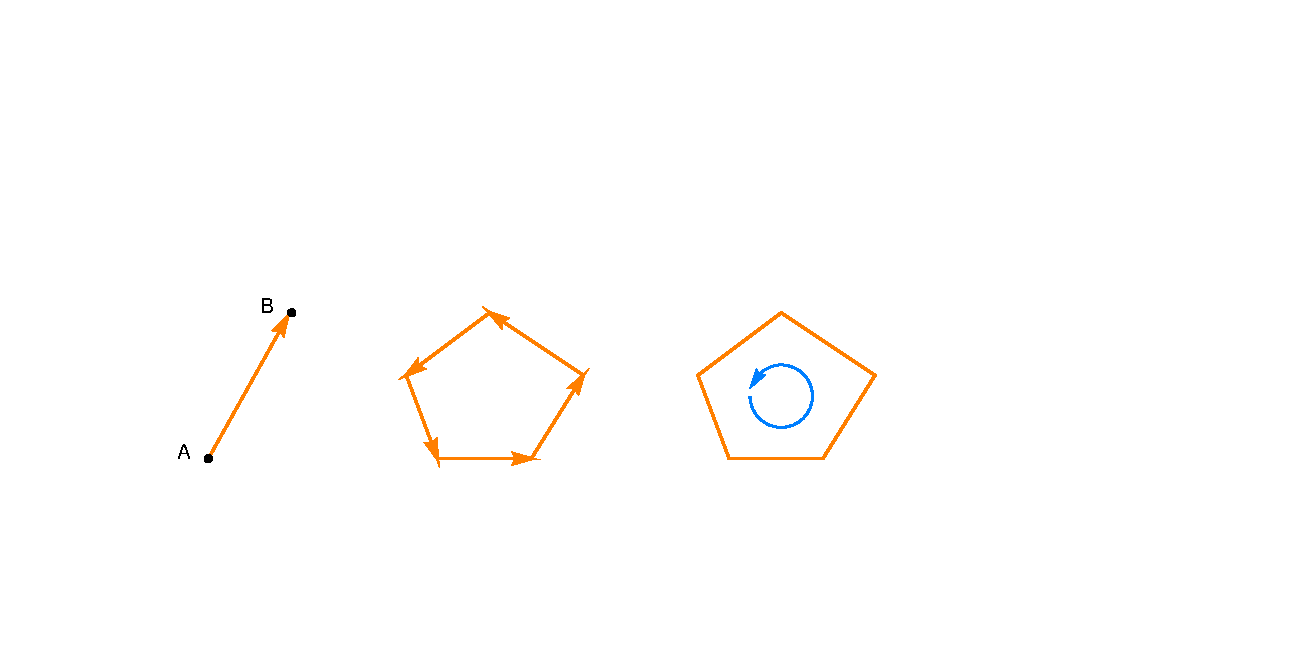
\includegraphics[width=90mm]{oriented-cells.eps}} }

We can think of an oriented segment as an arrow pointing from its negative extremity (base)
towards its positive extremity (tip).
We can think of an oriented polygon as having an arrow attached to each of it sides,
or we can imagine a small oriented circle inside the polygon.

\medskip
\centerline{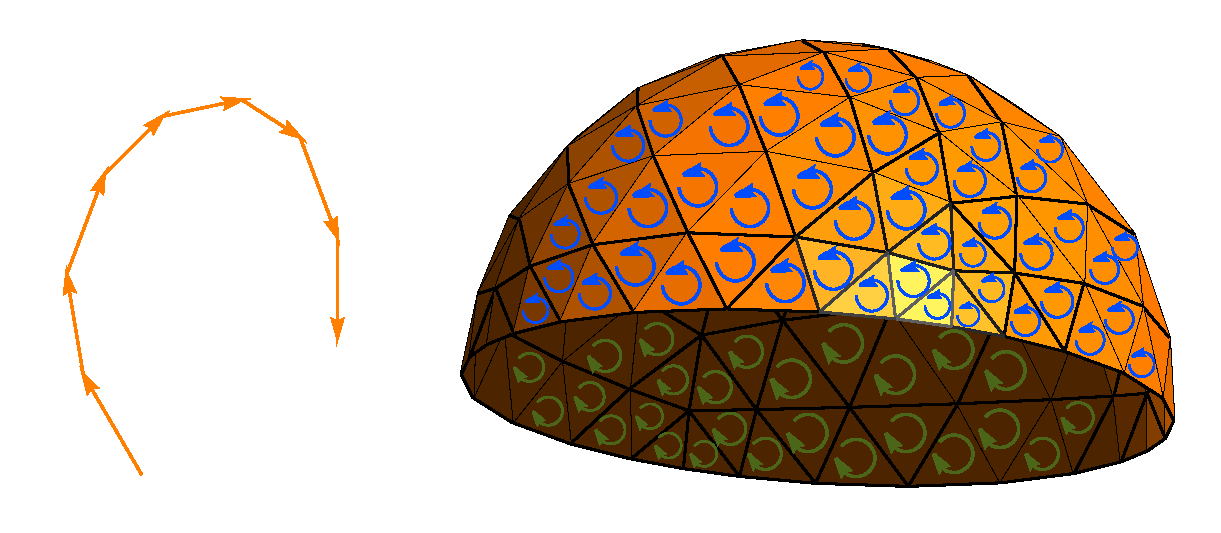
\includegraphics[width=110mm]{hemisphere-7.eps}}

A one-dimensional oriented mesh can be thought of as a chain of arrows,
each one pointing to the next segment's base (like in the drawing above right).
A two-dimensional oriented triangular mesh can be thought of as a web of triangles,
each triangle having a small oriented circle inside (like in the drawing above left).
The orientations of neighbour cells must be compatible : each segment must be seen
in opposite orientations from the point of view of its two neighbour triangles.

The above description of the orientation of a two-dimensional mesh does not depend
on the surrounding space.
A mesh can be immersed in some Euclidian space $ \RR^d $ or not.
In the case of a two-dimensional mesh immersed in $ \RR^3 $, the right hand rule establishes
a correspondence between the oriented circle described above and an arrow normal to the
surface being meshed.
Note, however, that the right hand rule is a convention based on the assuption that
the surrounding space $ \RR^3 $ has a certain orientation.

\medskip
\centerline{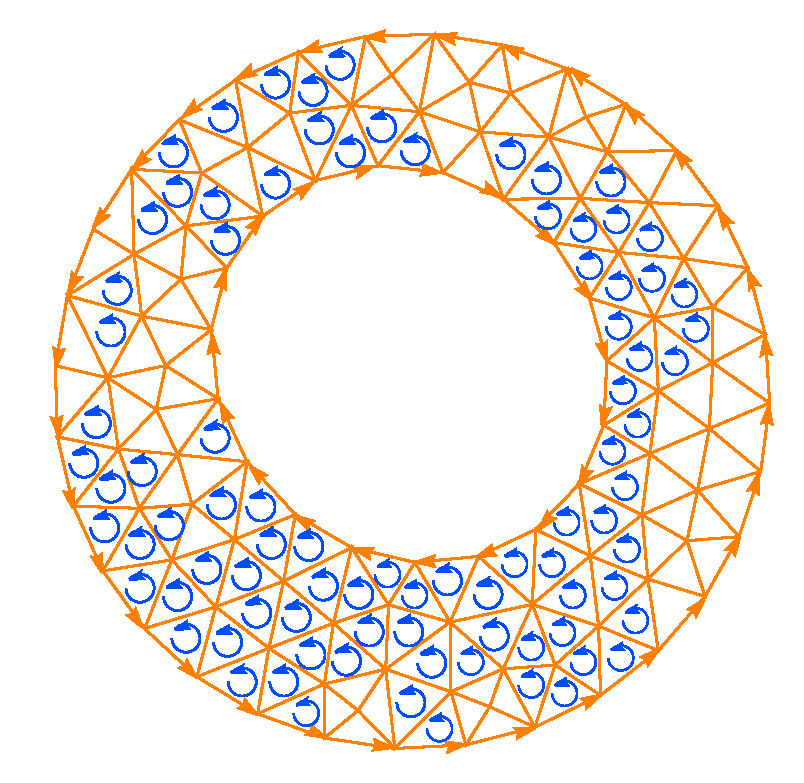
\includegraphics[width=75mm]{oriented-annulus-1.eps}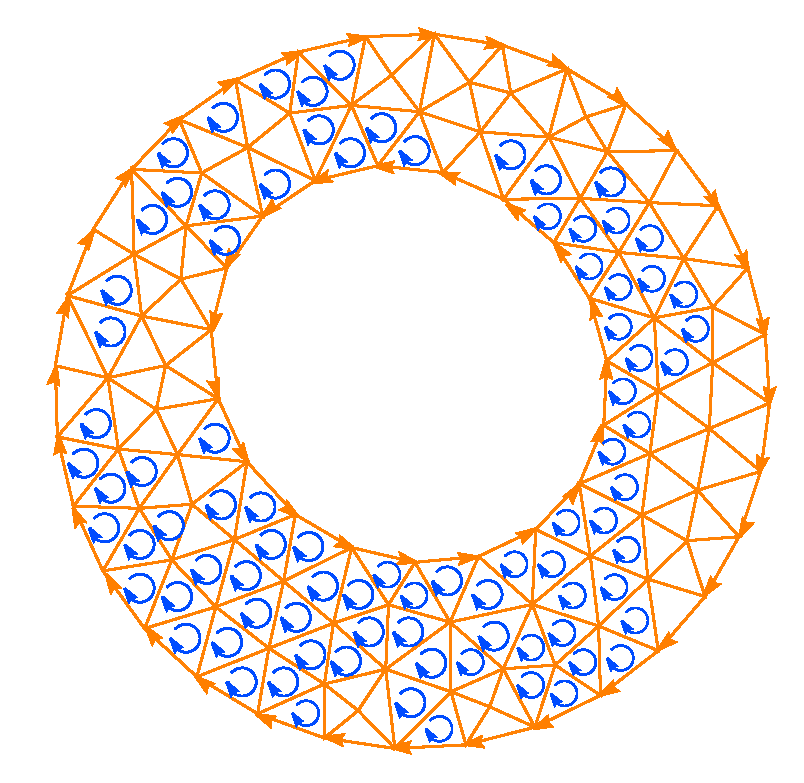
\includegraphics[width=75mm]{oriented-annulus-2.eps}}

Note also that an orientation of a mesh defines an orientation of its boundary.
In the above drawing we can see two opposite orientations of a mesh, together with
the corresponding orientation of its boundary.
This convention is used by Stokes' theorem.

Paragraphs \numb section 1.\numb parag 3 and \numb section 3.\numb parag 18 show examples where
the orientation of the boundary is important for joining meshes.

Cells have a {\codett reverse} method returning the reversed cell.
Segment {\codett Cell}s have methods {\codett base} and {\codett tip} returning their extremities.
For instance :

\verbatim
   Cell A ( tag::vertex );  Cell B ( tag::vertex );
   assert ( A.is_positive() );
   assert ( not A.reverse().is_positive() );
   assert ( A.reverse().reverse() == A );
   Cell AB ( tag::segment, A.reverse(), B );
   // here, AB is a segment Cell, not a Mesh
   assert ( AB.base() == A.reverse() );
   assert ( AB.tip() == B );
   Cell BA = AB.reverse();
   assert ( BA.base() == B.reverse() );
   assert ( BA.tip() == A );
   assert ( BA().reverse() == AB );
\endverbatim

Paragraph \numb section 8.\numb parag 7 gives more details about the orientation of cells.
See also paragraph \numb section 10.\numb parag 3.

Cells are topological entities; they carry no geometric information.
In particular, points do not have coordinates.
Coordinates are stored externally, see paragraph~\numb section 6.\numb parag 1.

{\codett Mesh}es have a {\codett reverse} method, too.
It is used mainly when we want to {\codett join} meshes having a common piece of boundary;
see e.g.\ paragraph \numb section 1.\numb parag 3.


\paragraph{\numb section 1.\numb parag 3. Joining meshes}

The example in paragraph~\numb section 1.\numb parag 1 could have been shortened had we used 
the overloaded version of the {\codett Mesh} constructor with {\codett tag::rectangle} which
accepts the four corners as arguments. 
This overloaded version exists in \maniFEM, but we prefer to build meshes in a structured way, 
first corners, then sides and then the plane region. 
This has the advantage that one can build more complex meshes from simple components. 
For instance, one can build an L-shaped mesh by joining three rectangular meshes :

\verbatim
   Manifold RR2 ( tag::Euclid, tag::of_dim, 2 );
   Function xy = RR2.build_coordinate_system ( tag::Lagrange, tag::of_degree, 1 );
   Function x = xy[0],  y = xy[1];
   Cell A ( tag::vertex );  x(A) = -1.;  y(A) = 0.;
   Cell B ( tag::vertex );  x(B) =  0.;  y(B) = 0.;
   Cell C ( tag::vertex );  x(C) =  0.;  y(C) = 0.5;
   Cell D ( tag::vertex );  x(D) = -1.;  y(D) = 0.5;
   Cell E ( tag::vertex );  x(E) =  0.;  y(E) = 1.;
   Cell F ( tag::vertex );  x(F) = -1.;  y(F) = 1.;
   Cell G ( tag::vertex );  x(G) =  1.;  y(G) = 0.;
   Cell H ( tag::vertex );  x(H) =  1.;  y(H) = 0.5;
   Mesh AB ( tag::segment, A.reverse(), B, tag::divided_in, 10 );
   Mesh BC ( tag::segment, B.reverse(), C, tag::divided_in, 8 );
   Mesh CD ( tag::segment, C.reverse(), D, tag::divided_in, 10 );
   Mesh DA ( tag::segment, D.reverse(), A, tag::divided_in, 8 );
   Mesh CE ( tag::segment, C.reverse(), E, tag::divided_in, 7 );
   Mesh EF ( tag::segment, E.reverse(), F, tag::divided_in, 10 );
   Mesh FD ( tag::segment, F.reverse(), D, tag::divided_in, 7 );
   Mesh BG ( tag::segment, B.reverse(), G, tag::divided_in, 12 );
   Mesh GH ( tag::segment, G.reverse(), H, tag::divided_in, 8 );
   Mesh HC ( tag::segment, H.reverse(), C, tag::divided_in, 12 );
   Mesh ABCD ( tag::rectangle, AB, BC, CD, DA );
   Mesh CEFD ( tag::rectangle, CE, EF, FD, CD.reverse() );
   Mesh BGHC ( tag::rectangle, BG, GH, HC, BC.reverse() );
   Mesh L_shaped ( tag::join, ABCD, CEFD, BGHC );
\endverbatim

{ \psfrag{A}{\special{ps: gsave 0 0 0.8 setrgbcolor}{\codett A}\special{ps: grestore}}
\psfrag{B}{\special{ps: gsave 0 0 0.8 setrgbcolor}{\codett B}\special{ps: grestore}}
\psfrag{C}{\special{ps: gsave 0 0 0.8 setrgbcolor}{\codett C}\special{ps: grestore}}
\psfrag{D}{\special{ps: gsave 0 0 0.8 setrgbcolor}{\codett D}\special{ps: grestore}}
\psfrag{E}{\special{ps: gsave 0 0 0.8 setrgbcolor}{\codett E}\special{ps: grestore}}
\psfrag{F}{\special{ps: gsave 0 0 0.8 setrgbcolor}{\codett F}\special{ps: grestore}}
\psfrag{G}{\special{ps: gsave 0 0 0.8 setrgbcolor}{\codett G}\special{ps: grestore}}
\psfrag{H}{\special{ps: gsave 0 0 0.8 setrgbcolor}{\codett H}\special{ps: grestore}}
\centerline{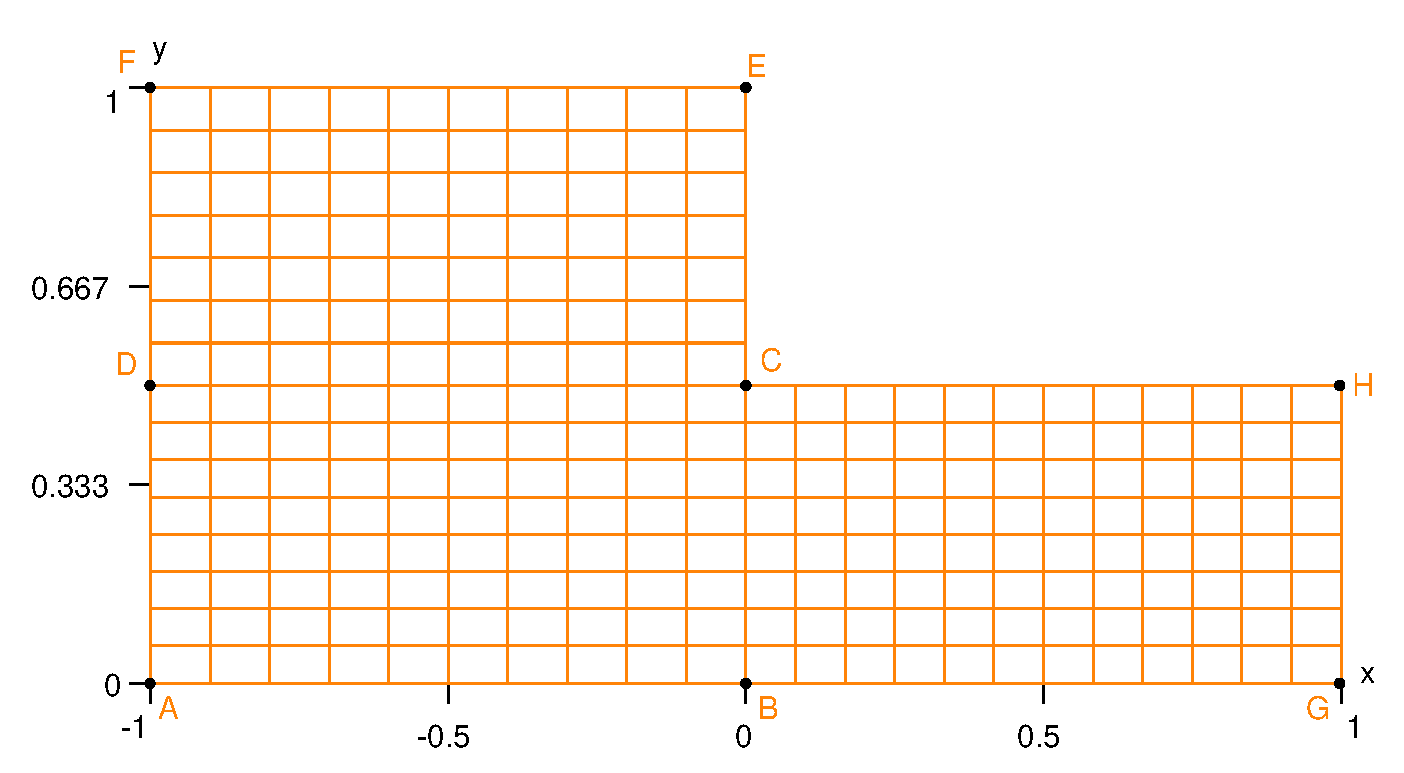
\includegraphics[width=10cm]{L-shaped.eps}} }

Meshes in $ \RR^2 $ like the one above may be exported in the {\codett msh} format
or directly drawn in {\codett Postcript}, by one of the two statements below

\verbatim
   L_shaped.export_msh ("L-shaped.msh");
   L_shaped.draw_ps ("L-shaped.eps");
\endverbatim

Note that, in \maniFEM, cells and meshes are oriented.
To build {\codett CEFD} one must use not {\codett CD} but its reverse;
to build {\codett BGHC} one must use not {\codett BC} but its reverse.

Note also that if we define the rectangles based on their vertices instead of their sides, 
the {\codett Mesh} constructor with {\codett tag::join} does not work properly. 
For instance, the two rectangles defined by

\verbatim
   Mesh ABCD ( tag::rectangle, A, B, C, D, 10, 8 );
   Mesh CEFD ( tag::rectangle, C, E, F, D, 7, 10 );
\endverbatim

\noindent cannot be joined%
\footnote *{\parbox{\ftntfont\baselineskip=3pt
Actually, they can be joined but the resulting mesh will have
a crack along {\ftnttt CD} -- probably not what the user wants.}}
because the side {\codett CD} of {\codett ABCD} has nothing to do with the side 
{\codett DC} of {\codett CEFD}.
These two sides are one-dimensional meshes both made of 10 segments but with different
interior points (only {\codett C} and {\codett D} are shared) and different segments.
In contrast, {\codett CD} and {\codett CD.reverse()} share the same 11 points and
the same 10 segments (reversed).

See paragraph \numb section 8.\numb parag 2 for a more complex use of the {\codett Mesh}
constructor with {\codett tag::join}.

Incidentally, note that the {\codett Mesh} constructor with {\codett tag::rectangle} accepts
any position for the vertices. 
Thus, you can use it to build any quadrilateral; the inner vertices' coordinates are simply
interpolated from the coordinates of vertices on the boundary, as shown in paragraphs
\numb section 1.\numb parag 5 and \numb section 2.\numb parag 1.
This can be done even in more than two (geometric) dimensions,
like in paragraphs \numb section 1.\numb parag 1 and \numb section 2.\numb parag 6.
Tags {\codett rectangle}, {\codett quadrilateral} and {\codett quadrangle} can be used
interchangeably.

See also paragraph \numb section 10.\numb parag 8.


\paragraph{\numb section 1.\numb parag 4. Triangular meshes}

We can also build meshes on triangular domains and {\codett join} them as we wish :

\verbatim
   Cell A ( tag::vertex );  x(A) = -1. ;  y(A) = 0.;
   Cell B ( tag::vertex );  x(B) =  0. ;  y(B) = 0.;
   Cell C ( tag::vertex );  x(C) =  1. ;  y(C) = 0.;
   Cell D ( tag::vertex );  x(D) = -0.5;  y(D) = 1.;
   Cell E ( tag::vertex );  x(E) =  0.5;  y(E) = 1.;
   Mesh AB ( tag::segment, A.reverse(), B, tag::divided_in, 8 );
   Mesh BC ( tag::segment, B.reverse(), C, tag::divided_in, 8 );
   Mesh AD ( tag::segment, A.reverse(), D, tag::divided_in, 8 );
   Mesh BD ( tag::segment, B.reverse(), D, tag::divided_in, 8 );
   Mesh BE ( tag::segment, B.reverse(), E, tag::divided_in, 8 );
   Mesh CE ( tag::segment, C.reverse(), E, tag::divided_in, 8 );
   Mesh ED ( tag::segment, E.reverse(), D, tag::divided_in, 8 );
   Mesh ABD ( tag::triangle, AB, BD, AD.reverse() );
   Mesh BCE ( tag::triangle, BC, CE, BE.reverse() );
   Mesh BED ( tag::triangle, BE, ED, BD.reverse() );
   Mesh three_tri ( tag::join, ABD, BCE, BED );
\endverbatim

{ \psfrag{A}{\special{ps: gsave 0 0 0.8 setrgbcolor}{\codett A}\special{ps: grestore}}
\psfrag{B}{\special{ps: gsave 0 0 0.8 setrgbcolor}{\codett B}\special{ps: grestore}}
\psfrag{C}{\special{ps: gsave 0 0 0.8 setrgbcolor}{\codett C}\special{ps: grestore}}
\psfrag{D}{\special{ps: gsave 0 0 0.8 setrgbcolor}{\codett D}\special{ps: grestore}}
\psfrag{E}{\special{ps: gsave 0 0 0.8 setrgbcolor}{\codett E}\special{ps: grestore}}
\centerline{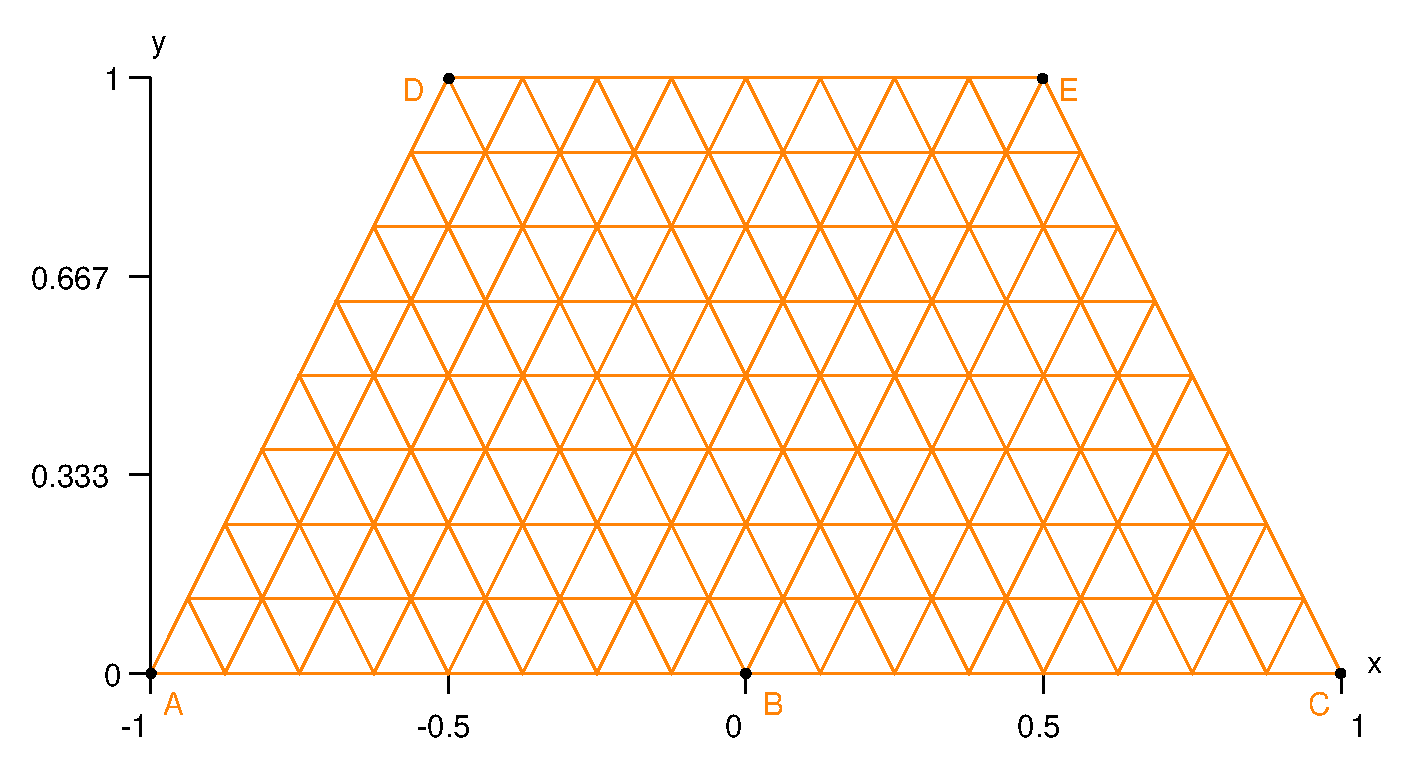
\includegraphics[width=9cm]{three-tri.eps}} }


\paragraph{\numb section 1.\numb parag 5. Mixing triangles and rectangles}

It is possible to have triangles and quadrilaterals mixed in the same mesh :

{ \psfrag{A}{\special{ps: gsave 0 0 0.8 setrgbcolor}{\codett A}\special{ps: grestore}}
\psfrag{B}{\special{ps: gsave 0 0 0.8 setrgbcolor}{\codett B}\special{ps: grestore}}
\psfrag{C}{\special{ps: gsave 0 0 0.8 setrgbcolor}{\codett C}\special{ps: grestore}}
\psfrag{D}{\special{ps: gsave 0 0 0.8 setrgbcolor}{\codett D}\special{ps: grestore}}
\psfrag{E}{\special{ps: gsave 0 0 0.8 setrgbcolor}{\codett E}\special{ps: grestore}}
\psfrag{F}{\special{ps: gsave 0 0 0.8 setrgbcolor}{\codett F}\special{ps: grestore}}
\centerline{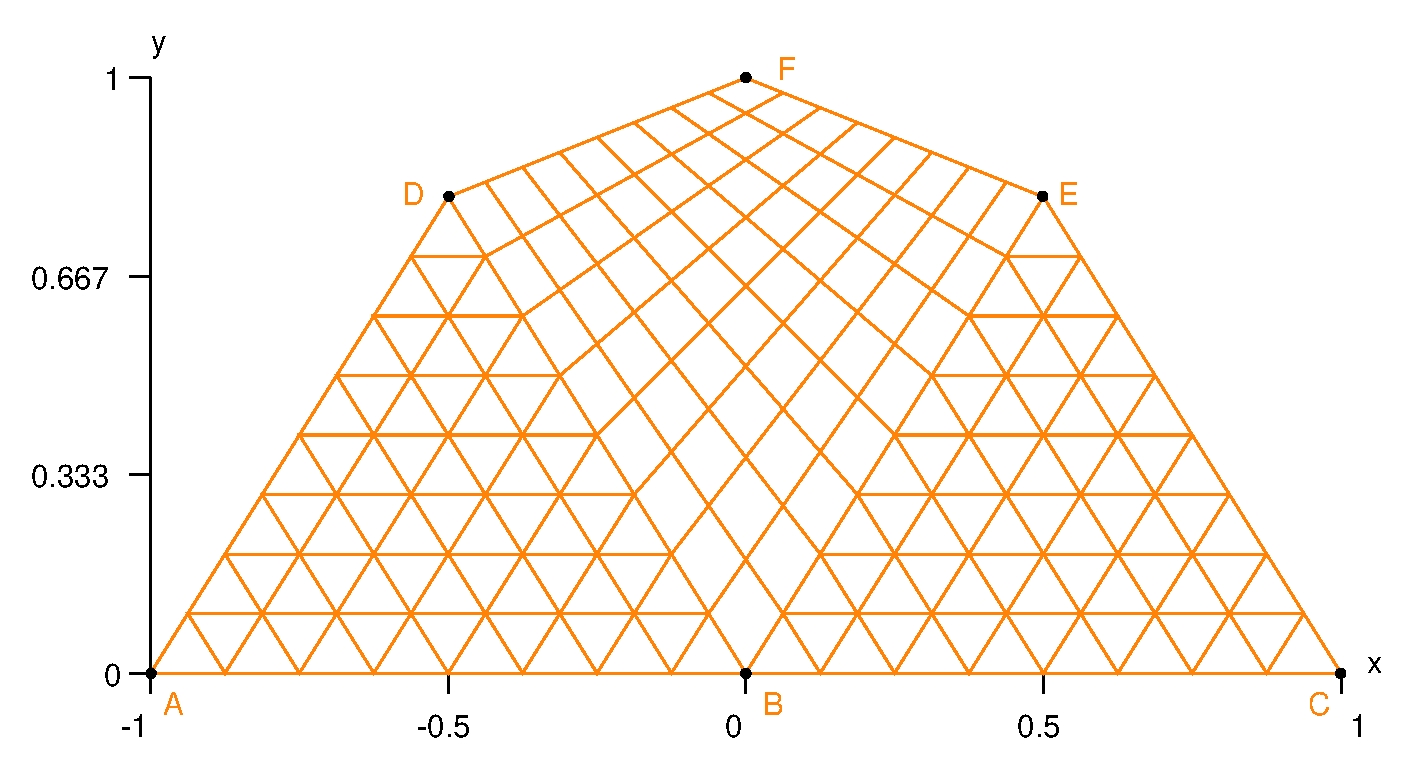
\includegraphics[width=95mm]{two-tri-one-rect.eps}} }

\verbatim
   Mesh ABD ( tag::triangle, AB, BD, AD.reverse() );
   Mesh BCE ( tag::triangle, BC, CE, BE.reverse() );
   Mesh BEFD ( tag::quadrangle, BE, EF, FD, BD.reverse() );
   Mesh two_tri_one_rect ( tag::join, ABD, BEFD, BCE );
\endverbatim

Paragraph \numb section 2.\numb parag 2 shows another example of mixed mesh.


\paragraph{\numb section 1.\numb parag 6. Functions}

Objects like {\codett xyz} and {\codett x} encountered in previous paragraphs
are {\codett Function} objects.
They allow for arithmetic expressions like in

\verbatim
   Function norm = power ( x*x + y*y, 0.5 );
\endverbatim

We access the value of a {\codett Function} at a cell like in {\codett double n = norm(A)}.
We can also set this value but not for arithmetic expressions like {\codett norm}.
Thus, pieces of code like {\codett x(A) = 1.} work fine, while {\codett norm(A) = 1.}
produces a run-time error.

The {\codett Function::deriv} method performs symbolic differentiation :

\verbatim
   Function norm_x = norm.deriv ( x );
   Function norm_y = norm.deriv ( y );
\endverbatim


